% Created 2021-10-21 qui 00:14
% Intended LaTeX compiler: pdflatex
\documentclass[twocolumn, 12pt]{article}
\usepackage[utf8]{inputenc}
\usepackage[T1]{fontenc}
\usepackage{graphicx}
\usepackage{grffile}
\usepackage{longtable}
\usepackage{wrapfig}
\usepackage{rotating}
\usepackage[normalem]{ulem}
\usepackage{amsmath}
\usepackage{textcomp}
\usepackage{amssymb}
\usepackage{capt-of}
\usepackage{hyperref}
\usepackage{minted}
\usepackage{cleveref}
\usepackage{subfig}
\usepackage{mathtools}
\usepackage[left=0.35in,top=0.25in,right=0.35in,bottom=0.25in]{geometry}
\usepackage[no-math]{fontspec}
\setsansfont{Linux Libertine}
\renewcommand{\familydefault}{\sfdefault}
\newcommand{\hl}{\noindent\rule{\textwidth}{0.5pt}}
\newcommand{\ie}{\textit{i.e. }}
\newcommand{\eg}{\textit{e.g. }}
\newcommand{\round}[1]{\ensuremath{\lfloor#1\rceil}}
\newcommand{\acomment}[1]{\textcolor{violet}{\emph{[#1]}}}
\DeclarePairedDelimiter\ceil{\lceil}{\rceil}
\DeclarePairedDelimiter\floor{\lfloor}{\rfloor}
\author{Guilherme G. Haetinger}
\date{2021-10-21  \hl}
\title{Assignment 4 - INF01009  \\ Applying Textures and Texture filtering to Arbitrary Texture-enabled Models}
\hypersetup{
 pdfauthor={Guilherme G. Haetinger},
 pdftitle={Assignment 4 - INF01009  \\ Applying Textures and Texture filtering to Arbitrary Texture-enabled Models},
 pdfkeywords={},
 pdfsubject={},
 pdfcreator={Emacs 27.2 (Org mode 9.5)}, 
 pdflang={English}}
\begin{document}

\maketitle


\section{Introduction}
\label{sec:org0ecb256}

Textures have many uses in computer graphics. They can be used not
only for holding images, but also to hold data of any sort.

In most cases, it is necessary that these textures can have
data queried in continuous coordinates. Furthermore, these queries
can result artifacts also known as aliasing, which has been the
subject of many works and algorithms, \textbf{two} of which we'll be covering
in this report.

\section{New File Structure}
\label{sec:org7414bf4}

In this assignment, we were introduced a new 3D Model representation
file. In this format, we get an indicator of whether the model has
texture coordinates or not. My new implementation checks if the
model is receptive to texture and constructs the \emph{UI} without the
related buttons/options.

\section{Setting up Texture attributes}
\label{sec:org4299d73}

There are essentially two attributes related to the textures:
\begin{itemize}
\item The texture coordinates, which will be taken care \emph{per}
vertex. They will be set inside a vertex attribute buffer for
\textbf{OpenGL} and will be fed as an attribute to the \textbf{Close2GL}
vertices. In the latter, we must highlight that it is also divided
by the perspective correction;

\item The texture filtering mode, which will be set as an option in our
\texttt{Options} class, processed both by \textbf{OpenGL}, setting the texture
parameters to either:
\begin{itemize}
\item \texttt{GL\_NEAREST}: Nearest Neighbor;
\item \texttt{GL\_LINEAR}: Bilinear Interpolation;
\item \texttt{GL\_MIPMAP}: MipMap Pyramid with Trilinear Interpolation. It is
important to point out that we need to ask \textbf{OpenGL} to generate
the MipMapped layers.
\end{itemize}
\end{itemize}

\section{Close2GL Texture Filtering}
\label{sec:orgd1a79ae}

In this section, we'll go over the three asked features for
transforming continuous texture coordinates resulted from the scan
conversion process to color.

\subsection{Nearest Neighbor}
\label{sec:org43ac155}

This is the most simple way of fetching the texture color. For a
given continuous coordinate \(c\), we calculate the discrete
coordinate \(c_{nn} = \round{c}\). This coordinate will be use to
query a color from the texture.

\uline{What would happen if this is oversampled (more pixels than
coordinates)?} The answer is quite simple: We would have chunks of
sequential pixels with the same color, which would highlight even
more harsh color changes. Check out \cref{fig:NN}.

\uline{What would happen if this is undersampled (more coordinates than
coordinates)?} The image would turn pixelated and, depending on the
amount of detail, can become difficult to understand. Check out \cref{fig:zoomed-out}.

\begin{figure}[htbp]
\centering
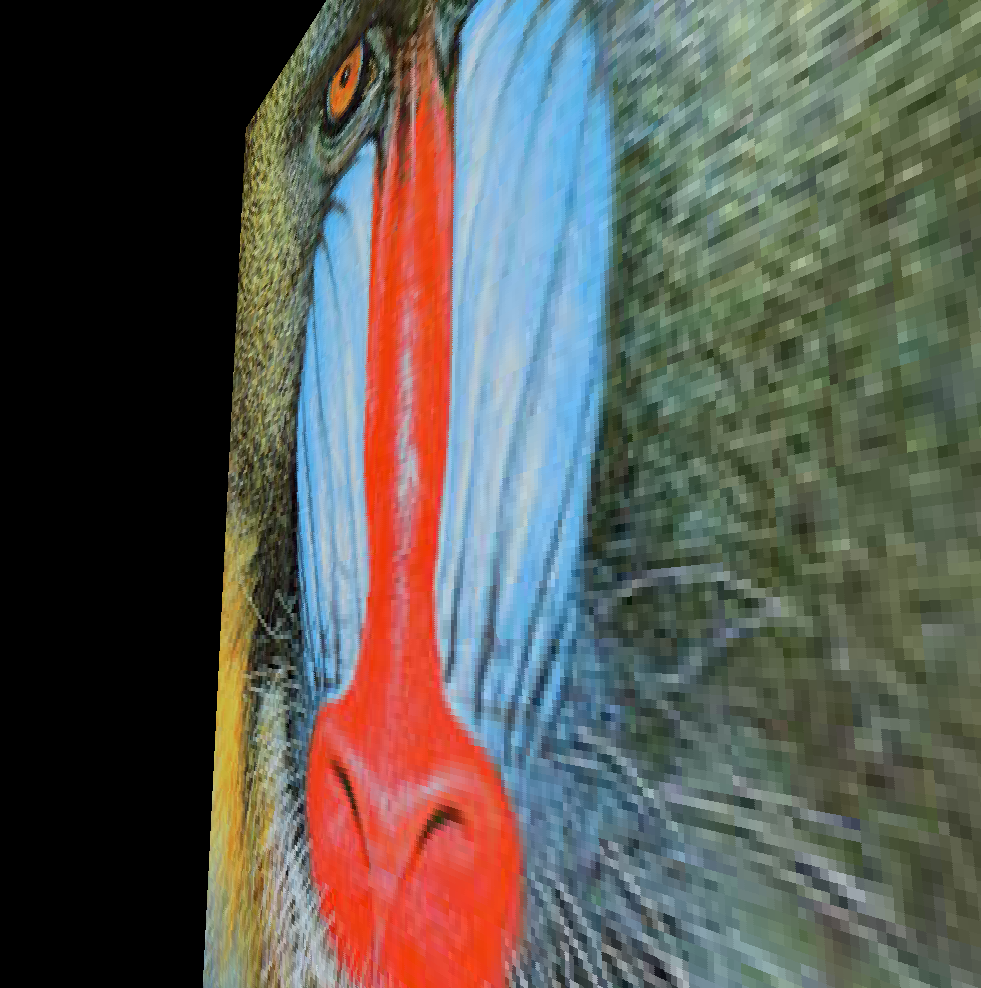
\includegraphics[width=\linewidth]{./res/NN-mandrill.png}
\caption{\label{fig:NN}Nearest Neighbor algorithm's harsh edges on top of the Mandrill image.}
\end{figure}

\subsection{Bilinear Interpolation}
\label{sec:orgd9673c7}

Bilinear interpolation helps us generate smooth gradients for
oversampled textures, removing harsh borders. The process is quite
simple, for continuous coordinate \(C\):

\begin{align*}
  a &= \begin{bmatrix}
    \floor{c.x} \\
    \floor{c.y}
  \end{bmatrix},
  b = \begin{bmatrix}
    \ceil{c.x} \\
    \floor{c.y}
  \end{bmatrix},
  c = \begin{bmatrix}
    \floor{c.x} \\
    \floor{c.y}
  \end{bmatrix},
  d = \begin{bmatrix}
    \ceil{c.x} \\
    \ceil{c.y}
  \end{bmatrix} \\
  ab &= (C.x - a.x) * a.color + (1 - (C.x - a.x)) * b.color \\
  cd &= (C.x - c.x) * c.color + (1 - (C.x - c.x)) * d.color \\
  color &= (C.y - a.y) * ab + (1 - (C.x - a.x)) * cd
\end{align*}

By the end, we'll have a very smooth surface not very prone to
harsh color changes when oversampled \cref{fig:Bilinear}. It still suffers from
aliasing when undersampled, however!

\begin{figure}[htbp]
\centering
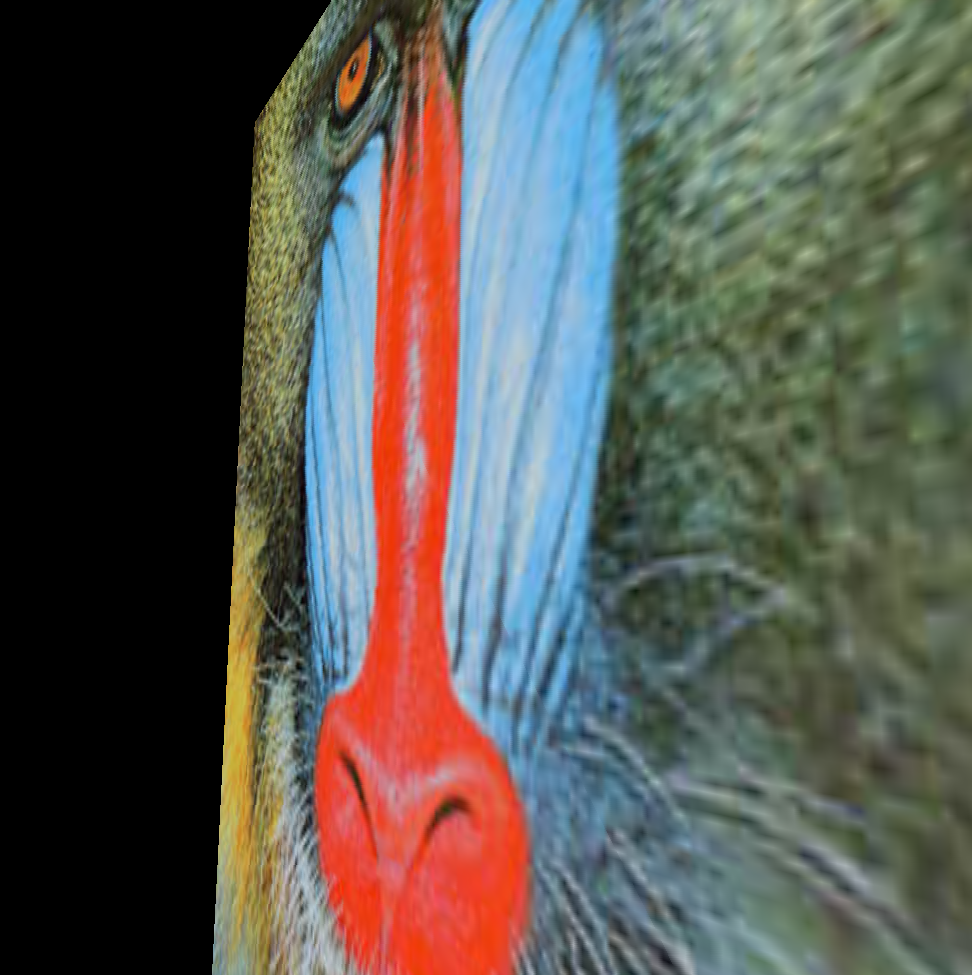
\includegraphics[width=\linewidth]{./res/Bilinear-mandrill.png}
\caption{\label{fig:Bilinear}Bilinear algorithm's smooth edges on top of the Mandrill image.}
\end{figure}

\subsection{MipMapped Trilinear Interpolation}
\label{sec:org73fa269}

Mipmapping can be done by constructing a pyramid of images, each
level having a degree of \emph{blurriness} generated by calculating a
mean of the closest 4 points. We, then, use levels of lower
resolution to render points further away in the perspective deform,
\ie points that ocuppy space that would be mapped to more than one
pixel (undersampling). By dynamically changing the level of the
texture fed to the viewport, we get a much moother perspective
result. We do so by applying \textbf{Trilinear Interpolation}, which is
basically doing the Bilinear interpolation on two mip levels and
interpolating between them.

    \begingroup
    \begin{figure}
    \captionsetup[subfigure]{justification=centering}
    \centering
    \label{fig:angle}
    \caption{Mipmap angled result (a) compared to Bilinear angled result (b). It is
clear the Mipmapped image  is clearer even from an angle.}
    \subfloat[]{\label{fig:angmip}%
    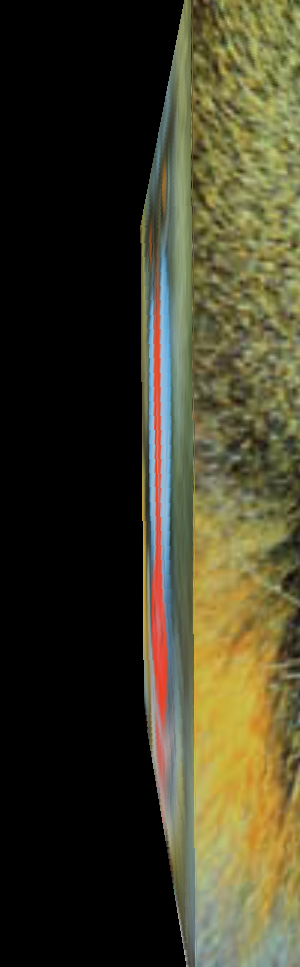
\includegraphics[width=0.48\linewidth, height=0.48\linewidth]{res/angled-mipmap}}%
    \hspace{0.1em}%
    \subfloat[]{\label{fig:angbil}%
    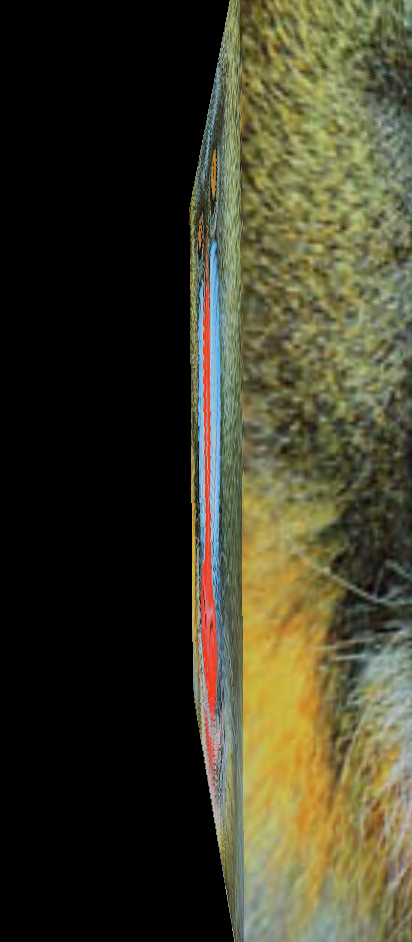
\includegraphics[width=0.48\linewidth, height=0.48\linewidth]{res/angled-bilinear}}%
    \end{figure}
    \endgroup

\begingroup
\begin{figure}
\captionsetup[subfigure]{justification=centering}
\centering
\label{fig:zoomed-out}
\caption{Zoomed out textures to compare how they behave while undersampled. It's clear (c) holds the advantage.}
\subfloat[Nearest Neighbor]{\label{fig:zoomnn}%
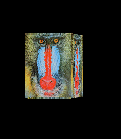
\includegraphics[width=0.33\linewidth, height=0.48\linewidth]{res/zoomed-out-nn}}%
\hspace{0.1em}%
\subfloat[Bilinear]{\label{fig:zoombl}%
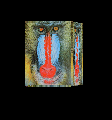
\includegraphics[width=0.33\linewidth, height=0.48\linewidth]{res/zoomed-out-bilinear}}%
\hspace{0.1em}%
\subfloat[Mipmapped]{\label{fig:zoommpmp}%
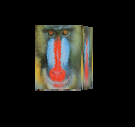
\includegraphics[width=0.33\linewidth, height=0.48\linewidth]{res/zoomed-out-mipmap}}%
\end{figure}
\endgroup

\section{Texture Modulate Shading}
\label{sec:orge93d54d}

We add the texture process organically, meaning the texture color will replace
the original object color from the previous assignments. However, this makes
us keep track and perspective divide attributes such as the diffuse
coefficient and the specular component for every vertex in the Gouraud model.

\begingroup
\begin{figure}
\captionsetup[subfigure]{justification=centering}
\centering
\label{fig:lights}
\caption{All lighting models required. Obs.: The cube might not have been the best model to show these off.}
\subfloat[Gourad (- Specularity)]{\label{fig:gourad-spec}%
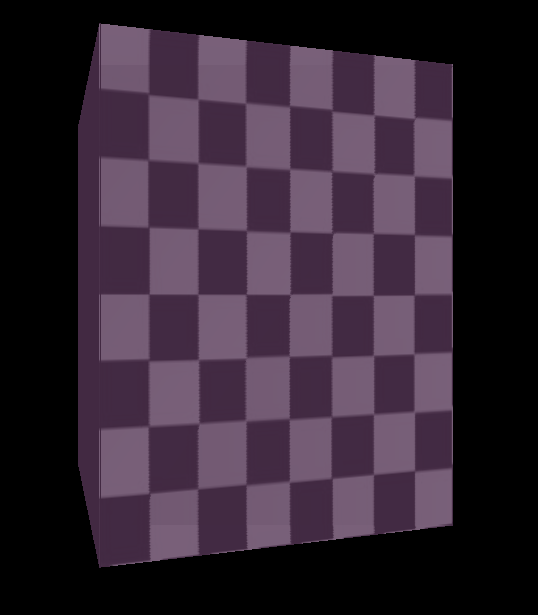
\includegraphics[width=0.33\linewidth, height=0.48\linewidth]{res/gourad-spec}}%
\hspace{0.1em}%
\subfloat[Gourad]{\label{fig:gourad}%
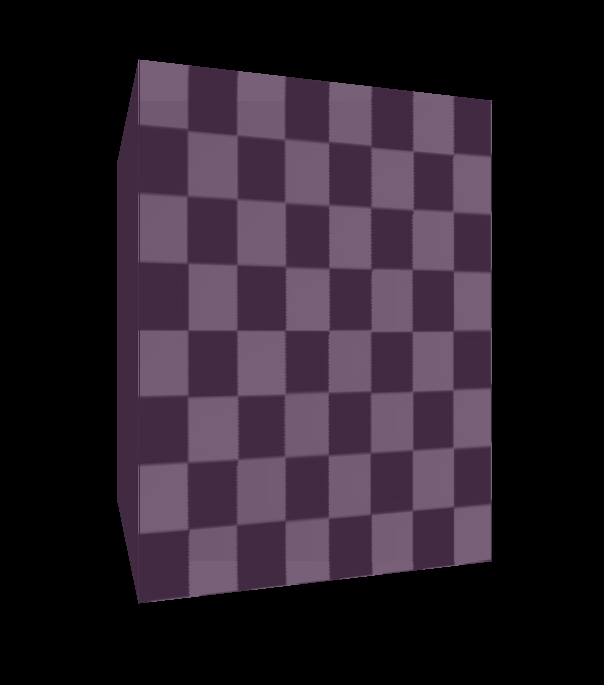
\includegraphics[width=0.33\linewidth, height=0.48\linewidth]{res/gourad}}%
\hspace{0.1em}%
\subfloat[Phong]{\label{fig:phong}%
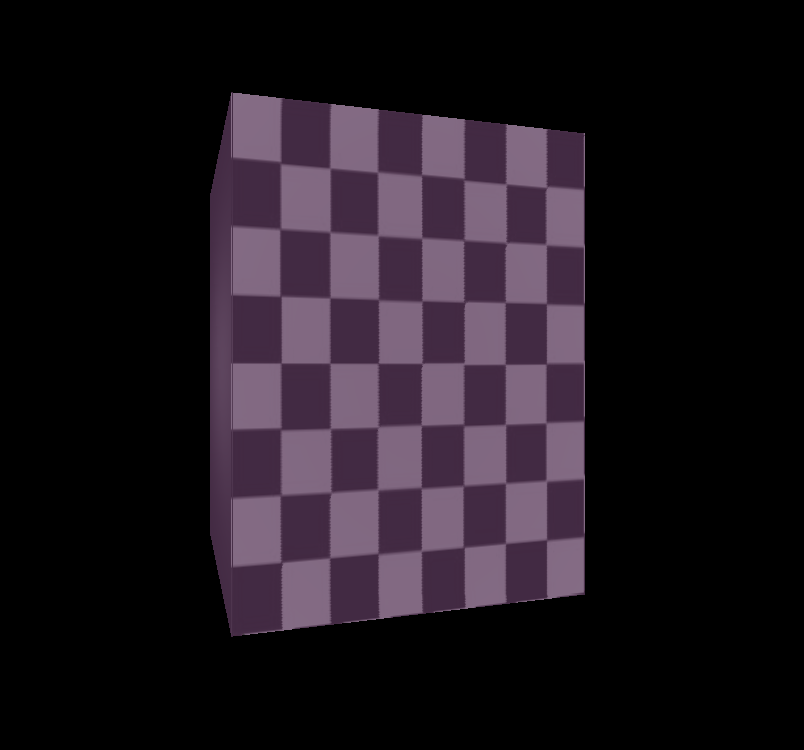
\includegraphics[width=0.33\linewidth, height=0.48\linewidth]{res/phong}}%
\end{figure}
\endgroup

\section{Conclusions}
\label{sec:org4b6672f}

This was definitely the easiest project of them all. There was definitely a bit
of a learning curve both on the mipmapping attribute definition and on the
calculation of the Pyramid. I really liked the results. I've also liked how my
result compares to \textbf{OpenGL}'s (\cref{fig:opengl}).

There are somethings I might need to fix regarding edge cases. I've also bumped
the speed of the program to over \uline{30FPS} using Phong shading!

\begingroup
\begin{figure}
\captionsetup[subfigure]{justification=centering}
\centering
\label{fig:opengl}
\caption{Close2GL mipmapping Vs. OpenGL's Mipmap result.}
\subfloat[Close2GL]{\label{fig:close}%
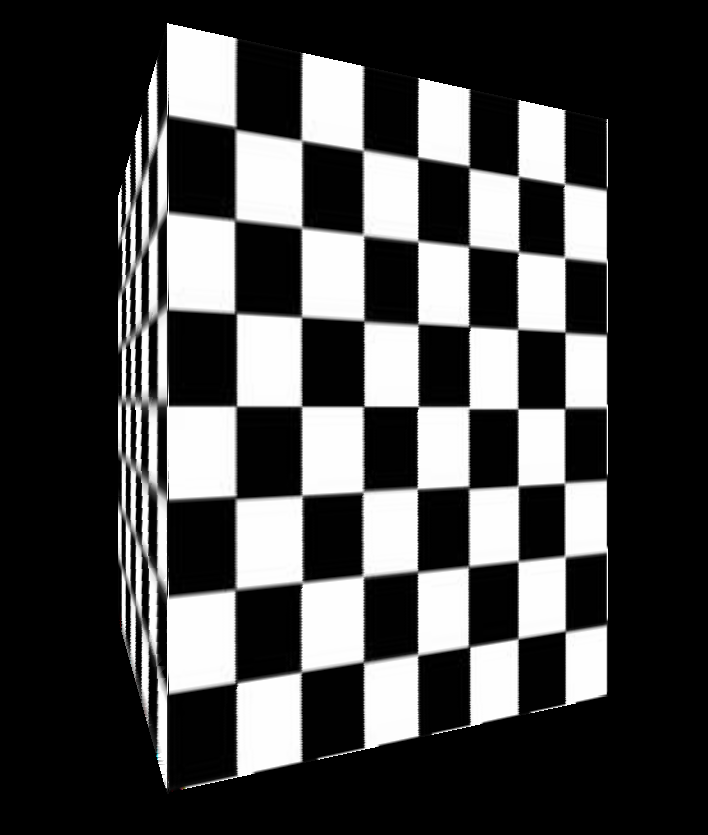
\includegraphics[width=0.48\linewidth, height=0.48\linewidth]{res/close2gl-checkers}}%
\hspace{0.1em}%
\subfloat[OpenGL]{\label{fig:open}%
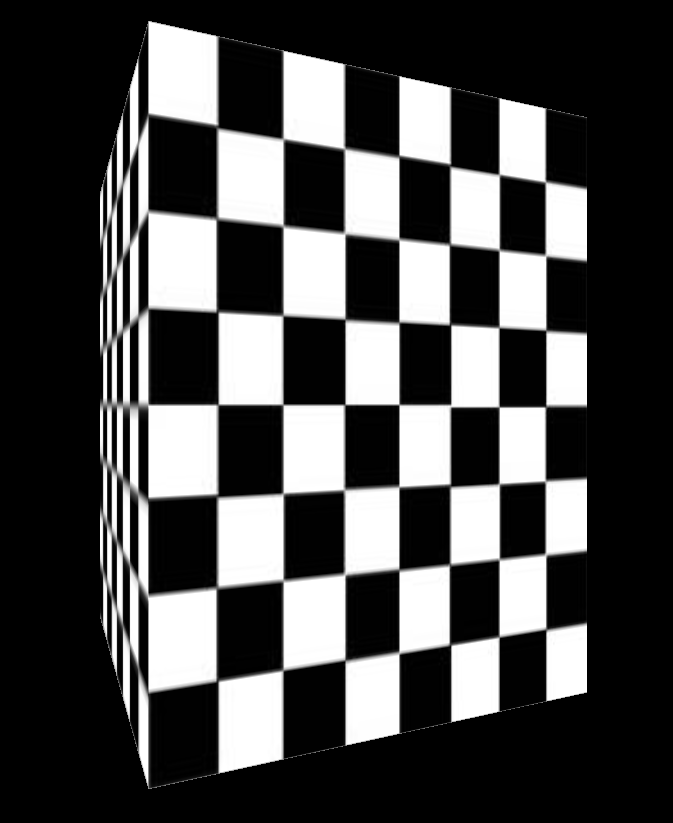
\includegraphics[width=0.48\linewidth, height=0.48\linewidth]{res/opengl-checkers}}%
\end{figure}
\endgroup
\end{document}
